%
		\subsection{Bohm Criteria}\label{sec:bohmcriteria}
%		
			To calculate the exact velocity at which an ion is entering the plasma sheath, the equation of motion has to be solved. Therefore the ion and electron densities from~\autoref{equ:ionandelectrondens} are substituted into \emph{Poisson's}~\autoref{equ:pseudo}. This is shown in~\autoref{equ:inequality}.\\		
			Because we know that the acceleration of an ion increases with decreasing distance to the wall --- therefore we will take a look at the expression for $\Phi(x)$ in~\autoref{equ:langmuirpot}, which yields $\Delta\Phi\le0$ and therefore $\nabla E \le0$. Therefore the potential derivative of the function $f(\Phi)$ at the sheath-boundary, e.g\@ $\Phi=0$, is analoguous to the gradient of the electric field in the Maxwell's equation.
%
			\begin{align} 
				f{\left(\Phi\right)}=%
					\Delta_{\vec{r}}\Phi=\frac{\diff^{2}\Phi}{\diff\vec{r}^{2}}=%
					\frac{\rho}{\varepsilon\ix{0}}%
				    \label{equ:pseudo}%\\[0.2cm]%
			\end{align}\vspace*{-18pt}\begin{align}
				0>\left.\frac{\diff f}{\diff\Phi}\right|_{\Phi=0}=%
					\frac{en\ix{e}\left(-d\right)}{\varepsilon\ix{0}}\left(\frac{e}%
					{k\ix{b}T\ix{e}}-\frac{e}{m\ix{i}v\ix{i,0}^{2}}\right)%
%					\nonumber\\[0.2cm]%
                \quad\Rightarrow\quad%
					v\ix{i,0}=v\ix{i,B}\ge\sqrt{\frac{k\ix{B}T\ix{e}}{m\ix{i}}}%
					\label{equ:inequality}
			\end{align}
%
			\begin{figure}[!b]
				\centering%
				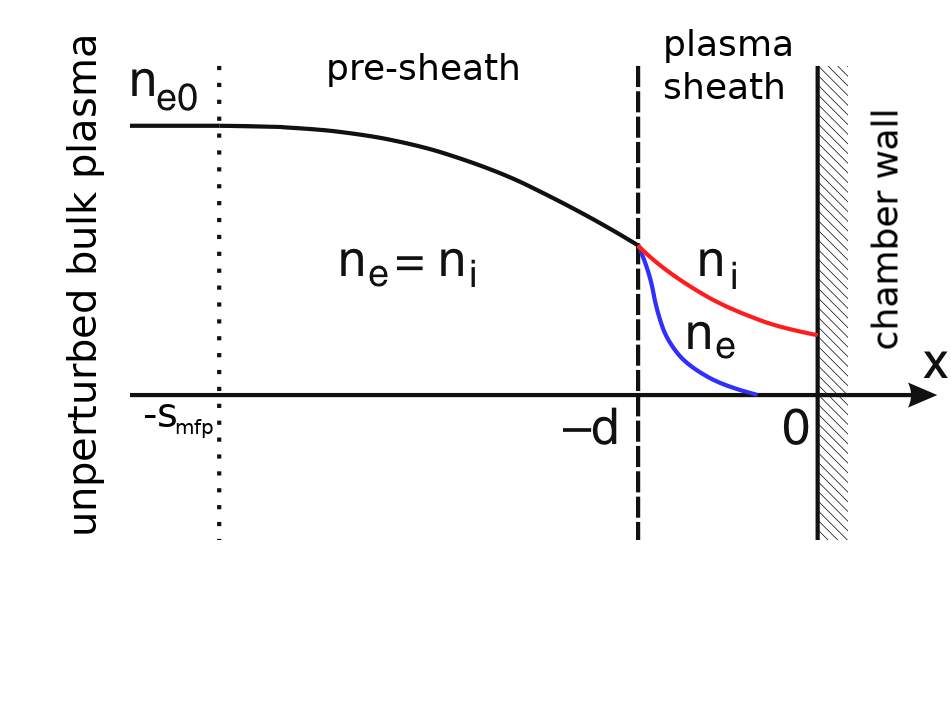
\includegraphics[width=0.6\textwidth]{figures/sheath_piel.png}%
				\caption{%
				One dimensional density profiles as a function of the distance to a floating wall. Note the exponential decrease of the electron density $n\ix{e}$ from the sheath border towards the negatively charged wall. Densities allready reach approximately 0.66$\cdot n\ix{e,0}$ inside the pre-sheath.~\cite{Piel10}}\label{fig:sheath_piel}
			\end{figure}
%	
			Analoguos you can define the so called \emph{Mach number} $M=v\ix{i,0}/v\ix{i,B}$, where $v\ix{i,B}$ denotes the \emph{Bohm velocity}. At the sheath-boundary the quasi-neutrality condition is still satisfied: $n\ix{e}=n\ix{i}\,$. The potential $\Phi{\left(x\right)}$ inside the pre-sheath from~\autoref{equ:langmuirpot} and the bulk ion density $n\ix{i,0}$ from~\autoref{equ:ionandelectrondens} are now used to describe the ion transport process in the pre-sheath. This is dominated by collisions with neutral gas particles, hence the velocity distribution function can be rewritten using the ion-neutral collisions frequency $\nu\ix{n,i}\,$.
%
			\begin{align}
				\frac{\diff v\ix{i}}{\diff x}=\frac{\nu\ix{n,i}v\ix{i}^{2}}{v\ix{B}^{2}-v\ix{i}^{2}}\quad.%
				\label{equ:distribution}
			\end{align}
%
			From~\autoref{equ:distribution} we can see: ions with velocities smaller than the Bohm velocity are accelerated inside the pre-sheath. According to~\autoref{equ:inequality} velocities greater than $v\ix{B}$ are not allowed. Hence the ion velocity is exactly $v\ix{B}$ at the boundary of the plasma sheath.
%
			\begin{align}
				M\ge1%
				\Leftrightarrow%
				v\ix{i}(-d)\ge v\ix{B}%
				\label{equ:bohmcriteria2}
			\end{align}
%
			At $x=-d$, both negative and positive charge density decreased to $n\ix{i}=n\ix{e}\approx\SI{0.66}n\ix{e,0}$ (see~\autoref{fig:sheath_piel}), where the potential is approximately $-k\ix{B}T\ix{e}/2e$ because of the currents onto the wall. In summary,the ion dynamic discussed before is spatially restricted to the sheath and pre-sheath. They only develop where there is electron depletion or an externally applied, negative potential.